% Options for packages loaded elsewhere
\PassOptionsToPackage{unicode}{hyperref}
\PassOptionsToPackage{hyphens}{url}
\PassOptionsToPackage{dvipsnames,svgnames,x11names}{xcolor}
%
\documentclass[
  letterpaper,
  DIV=11,
  numbers=noendperiod]{scrartcl}

\usepackage{amsmath,amssymb}
\usepackage{lmodern}
\usepackage{iftex}
\ifPDFTeX
  \usepackage[T1]{fontenc}
  \usepackage[utf8]{inputenc}
  \usepackage{textcomp} % provide euro and other symbols
\else % if luatex or xetex
  \usepackage{unicode-math}
  \defaultfontfeatures{Scale=MatchLowercase}
  \defaultfontfeatures[\rmfamily]{Ligatures=TeX,Scale=1}
\fi
% Use upquote if available, for straight quotes in verbatim environments
\IfFileExists{upquote.sty}{\usepackage{upquote}}{}
\IfFileExists{microtype.sty}{% use microtype if available
  \usepackage[]{microtype}
  \UseMicrotypeSet[protrusion]{basicmath} % disable protrusion for tt fonts
}{}
\makeatletter
\@ifundefined{KOMAClassName}{% if non-KOMA class
  \IfFileExists{parskip.sty}{%
    \usepackage{parskip}
  }{% else
    \setlength{\parindent}{0pt}
    \setlength{\parskip}{6pt plus 2pt minus 1pt}}
}{% if KOMA class
  \KOMAoptions{parskip=half}}
\makeatother
\usepackage{xcolor}
\setlength{\emergencystretch}{3em} % prevent overfull lines
\setcounter{secnumdepth}{5}
% Make \paragraph and \subparagraph free-standing
\ifx\paragraph\undefined\else
  \let\oldparagraph\paragraph
  \renewcommand{\paragraph}[1]{\oldparagraph{#1}\mbox{}}
\fi
\ifx\subparagraph\undefined\else
  \let\oldsubparagraph\subparagraph
  \renewcommand{\subparagraph}[1]{\oldsubparagraph{#1}\mbox{}}
\fi

\usepackage{color}
\usepackage{fancyvrb}
\newcommand{\VerbBar}{|}
\newcommand{\VERB}{\Verb[commandchars=\\\{\}]}
\DefineVerbatimEnvironment{Highlighting}{Verbatim}{commandchars=\\\{\}}
% Add ',fontsize=\small' for more characters per line
\usepackage{framed}
\definecolor{shadecolor}{RGB}{241,243,245}
\newenvironment{Shaded}{\begin{snugshade}}{\end{snugshade}}
\newcommand{\AlertTok}[1]{\textcolor[rgb]{0.68,0.00,0.00}{#1}}
\newcommand{\AnnotationTok}[1]{\textcolor[rgb]{0.37,0.37,0.37}{#1}}
\newcommand{\AttributeTok}[1]{\textcolor[rgb]{0.40,0.45,0.13}{#1}}
\newcommand{\BaseNTok}[1]{\textcolor[rgb]{0.68,0.00,0.00}{#1}}
\newcommand{\BuiltInTok}[1]{\textcolor[rgb]{0.00,0.23,0.31}{#1}}
\newcommand{\CharTok}[1]{\textcolor[rgb]{0.13,0.47,0.30}{#1}}
\newcommand{\CommentTok}[1]{\textcolor[rgb]{0.37,0.37,0.37}{#1}}
\newcommand{\CommentVarTok}[1]{\textcolor[rgb]{0.37,0.37,0.37}{\textit{#1}}}
\newcommand{\ConstantTok}[1]{\textcolor[rgb]{0.56,0.35,0.01}{#1}}
\newcommand{\ControlFlowTok}[1]{\textcolor[rgb]{0.00,0.23,0.31}{#1}}
\newcommand{\DataTypeTok}[1]{\textcolor[rgb]{0.68,0.00,0.00}{#1}}
\newcommand{\DecValTok}[1]{\textcolor[rgb]{0.68,0.00,0.00}{#1}}
\newcommand{\DocumentationTok}[1]{\textcolor[rgb]{0.37,0.37,0.37}{\textit{#1}}}
\newcommand{\ErrorTok}[1]{\textcolor[rgb]{0.68,0.00,0.00}{#1}}
\newcommand{\ExtensionTok}[1]{\textcolor[rgb]{0.00,0.23,0.31}{#1}}
\newcommand{\FloatTok}[1]{\textcolor[rgb]{0.68,0.00,0.00}{#1}}
\newcommand{\FunctionTok}[1]{\textcolor[rgb]{0.28,0.35,0.67}{#1}}
\newcommand{\ImportTok}[1]{\textcolor[rgb]{0.00,0.46,0.62}{#1}}
\newcommand{\InformationTok}[1]{\textcolor[rgb]{0.37,0.37,0.37}{#1}}
\newcommand{\KeywordTok}[1]{\textcolor[rgb]{0.00,0.23,0.31}{#1}}
\newcommand{\NormalTok}[1]{\textcolor[rgb]{0.00,0.23,0.31}{#1}}
\newcommand{\OperatorTok}[1]{\textcolor[rgb]{0.37,0.37,0.37}{#1}}
\newcommand{\OtherTok}[1]{\textcolor[rgb]{0.00,0.23,0.31}{#1}}
\newcommand{\PreprocessorTok}[1]{\textcolor[rgb]{0.68,0.00,0.00}{#1}}
\newcommand{\RegionMarkerTok}[1]{\textcolor[rgb]{0.00,0.23,0.31}{#1}}
\newcommand{\SpecialCharTok}[1]{\textcolor[rgb]{0.37,0.37,0.37}{#1}}
\newcommand{\SpecialStringTok}[1]{\textcolor[rgb]{0.13,0.47,0.30}{#1}}
\newcommand{\StringTok}[1]{\textcolor[rgb]{0.13,0.47,0.30}{#1}}
\newcommand{\VariableTok}[1]{\textcolor[rgb]{0.07,0.07,0.07}{#1}}
\newcommand{\VerbatimStringTok}[1]{\textcolor[rgb]{0.13,0.47,0.30}{#1}}
\newcommand{\WarningTok}[1]{\textcolor[rgb]{0.37,0.37,0.37}{\textit{#1}}}

\providecommand{\tightlist}{%
  \setlength{\itemsep}{0pt}\setlength{\parskip}{0pt}}\usepackage{longtable,booktabs,array}
\usepackage{calc} % for calculating minipage widths
% Correct order of tables after \paragraph or \subparagraph
\usepackage{etoolbox}
\makeatletter
\patchcmd\longtable{\par}{\if@noskipsec\mbox{}\fi\par}{}{}
\makeatother
% Allow footnotes in longtable head/foot
\IfFileExists{footnotehyper.sty}{\usepackage{footnotehyper}}{\usepackage{footnote}}
\makesavenoteenv{longtable}
\usepackage{graphicx}
\makeatletter
\def\maxwidth{\ifdim\Gin@nat@width>\linewidth\linewidth\else\Gin@nat@width\fi}
\def\maxheight{\ifdim\Gin@nat@height>\textheight\textheight\else\Gin@nat@height\fi}
\makeatother
% Scale images if necessary, so that they will not overflow the page
% margins by default, and it is still possible to overwrite the defaults
% using explicit options in \includegraphics[width, height, ...]{}
\setkeys{Gin}{width=\maxwidth,height=\maxheight,keepaspectratio}
% Set default figure placement to htbp
\makeatletter
\def\fps@figure{htbp}
\makeatother

\KOMAoption{captions}{tableheading}
\makeatletter
\@ifpackageloaded{tcolorbox}{}{\usepackage[many]{tcolorbox}}
\@ifpackageloaded{fontawesome5}{}{\usepackage{fontawesome5}}
\definecolor{quarto-callout-color}{HTML}{909090}
\definecolor{quarto-callout-note-color}{HTML}{0758E5}
\definecolor{quarto-callout-important-color}{HTML}{CC1914}
\definecolor{quarto-callout-warning-color}{HTML}{EB9113}
\definecolor{quarto-callout-tip-color}{HTML}{00A047}
\definecolor{quarto-callout-caution-color}{HTML}{FC5300}
\definecolor{quarto-callout-color-frame}{HTML}{acacac}
\definecolor{quarto-callout-note-color-frame}{HTML}{4582ec}
\definecolor{quarto-callout-important-color-frame}{HTML}{d9534f}
\definecolor{quarto-callout-warning-color-frame}{HTML}{f0ad4e}
\definecolor{quarto-callout-tip-color-frame}{HTML}{02b875}
\definecolor{quarto-callout-caution-color-frame}{HTML}{fd7e14}
\makeatother
\makeatletter
\makeatother
\makeatletter
\makeatother
\makeatletter
\@ifpackageloaded{caption}{}{\usepackage{caption}}
\AtBeginDocument{%
\ifdefined\contentsname
  \renewcommand*\contentsname{Table des matières}
\else
  \newcommand\contentsname{Table des matières}
\fi
\ifdefined\listfigurename
  \renewcommand*\listfigurename{Liste des Figures}
\else
  \newcommand\listfigurename{Liste des Figures}
\fi
\ifdefined\listtablename
  \renewcommand*\listtablename{Liste des Tables}
\else
  \newcommand\listtablename{Liste des Tables}
\fi
\ifdefined\figurename
  \renewcommand*\figurename{Figure}
\else
  \newcommand\figurename{Figure}
\fi
\ifdefined\tablename
  \renewcommand*\tablename{Table}
\else
  \newcommand\tablename{Table}
\fi
}
\@ifpackageloaded{float}{}{\usepackage{float}}
\floatstyle{ruled}
\@ifundefined{c@chapter}{\newfloat{codelisting}{h}{lop}}{\newfloat{codelisting}{h}{lop}[chapter]}
\floatname{codelisting}{Listing}
\newcommand*\listoflistings{\listof{codelisting}{Liste des Listings}}
\makeatother
\makeatletter
\@ifpackageloaded{caption}{}{\usepackage{caption}}
\@ifpackageloaded{subcaption}{}{\usepackage{subcaption}}
\makeatother
\makeatletter
\@ifpackageloaded{tcolorbox}{}{\usepackage[many]{tcolorbox}}
\makeatother
\makeatletter
\@ifundefined{shadecolor}{\definecolor{shadecolor}{rgb}{.97, .97, .97}}
\makeatother
\makeatletter
\makeatother
\ifLuaTeX
\usepackage[bidi=basic]{babel}
\else
\usepackage[bidi=default]{babel}
\fi
\babelprovide[main,import]{french}
% get rid of language-specific shorthands (see #6817):
\let\LanguageShortHands\languageshorthands
\def\languageshorthands#1{}
\ifLuaTeX
  \usepackage{selnolig}  % disable illegal ligatures
\fi
\IfFileExists{bookmark.sty}{\usepackage{bookmark}}{\usepackage{hyperref}}
\IfFileExists{xurl.sty}{\usepackage{xurl}}{} % add URL line breaks if available
\urlstyle{same} % disable monospaced font for URLs
\hypersetup{
  pdftitle={Import et export de données},
  pdfauthor={Hugues pecout},
  pdflang={fr},
  colorlinks=true,
  linkcolor={blue},
  filecolor={Maroon},
  citecolor={Blue},
  urlcolor={Blue},
  pdfcreator={LaTeX via pandoc}}

\title{Import et export de données}
\usepackage{etoolbox}
\makeatletter
\providecommand{\subtitle}[1]{% add subtitle to \maketitle
  \apptocmd{\@title}{\par {\large #1 \par}}{}{}
}
\makeatother
\subtitle{Les différents types et formats de données pris en charge par
R}
\author{Hugues pecout}
\date{03/02/2023}

\begin{document}
\maketitle
\ifdefined\Shaded\renewenvironment{Shaded}{\begin{tcolorbox}[breakable, enhanced, boxrule=0pt, borderline west={3pt}{0pt}{shadecolor}, interior hidden, sharp corners, frame hidden]}{\end{tcolorbox}}\fi

\renewcommand*\contentsname{Table des matières}
{
\hypersetup{linkcolor=}
\setcounter{tocdepth}{3}
\tableofcontents
}
\textbf{De nombreuses de fonctions (primitives ou non) permettent
d'importer et d'exporter des données de différents formats.}

\hypertarget{tableau-de-donnuxe9es}{%
\subsection{\texorpdfstring{\textbf{Tableau de
données}}{Tableau de données}}\label{tableau-de-donnuxe9es}}

\hypertarget{fichier-texte-simple}{%
\subsubsection{Fichier texte simple}\label{fichier-texte-simple}}

Un fichier texte simple (ou fichier texte brut) est un fichier dont le
contenu représente uniquement une suite de caractères. Il peut s'ouvrir
avec n'importe quel éditeur de texte et utilise nécessairement une forme
particulière de codage des caractères.

Plusieurs fonctions primitives permettent d'importer et d'exporter des
fichiers texte simples, comme les fichiers \textbf{csv}, \textbf{txt} ,
\textbf{tsv}\ldots{}

\hypertarget{import}{%
\paragraph{Import}\label{import}}

\begin{itemize}
\tightlist
\item
  \texttt{read.delim()} : fichiers délimités par un symbole quelconque
  et ``.'' en séparateur décimal
\item
  \texttt{read.delim2()} : fichiers délimités par un symbole quelconque
  et ``,'' en séparateur décimal
\item
  \texttt{read.table()} : pour des fichiers texte délimités par des
  espaces\\
\item
  \texttt{read.csv()} : pour des fichiers texte délimités par des
  virgules (format csv)
\item
  \texttt{read.csv2()} : pour des fichiers texte délimités par des
  points-virgules (format csv français)
\end{itemize}

Pour que l'import de données s'effectue correctement, il est parfois
nécessaire de renseigner plusieurs arguments, comme par exemple :

\textbf{header} = valeur logique qui indique si la première ligne
contient les noms des variables. \textbf{sep} = indique le caractère
utilisé comme séparateur de champ (ex : ``;'') \textbf{encoding} =
Chaîne de caractère qui précise l'encodage utilisé pour le fichier (ex :
``UTF-8'').

\begin{tcolorbox}[enhanced jigsaw, colframe=quarto-callout-important-color-frame, bottomtitle=1mm, colback=white, leftrule=.75mm, breakable, left=2mm, titlerule=0mm, toptitle=1mm, arc=.35mm, title=\textcolor{quarto-callout-important-color}{\faExclamation}\hspace{0.5em}{Important}, rightrule=.15mm, bottomrule=.15mm, toprule=.15mm, colbacktitle=quarto-callout-important-color!10!white, opacitybacktitle=0.6, opacityback=0, coltitle=black]

N'oubliez pas d'assigner le résultat dans un objet pour garder en
mémoire vos données importées.

\end{tcolorbox}

\begin{Shaded}
\begin{Highlighting}[]
\CommentTok{\# Exemple d\textquotesingle{}utilisation de read.table()}
\NormalTok{mon\_tableau  }\OtherTok{\textless{}{-}} \FunctionTok{read.table}\NormalTok{(}\AttributeTok{file =} \StringTok{"../data/DEV\_AFRICA\_2018/afrika\_don\_meta.csv"}\NormalTok{, }
                           \AttributeTok{header =} \ConstantTok{TRUE}\NormalTok{,}
                           \AttributeTok{sep=} \StringTok{";"}\NormalTok{,}
                           \AttributeTok{encoding =} \StringTok{"UTF{-}8"}\NormalTok{)}


\CommentTok{\# Le tableau importé est stocké dans un objet data.frame}
\FunctionTok{class}\NormalTok{(mon\_tableau)}
\end{Highlighting}
\end{Shaded}

\begin{verbatim}
[1] "data.frame"
\end{verbatim}

\hypertarget{export}{%
\paragraph{Export}\label{export}}

Des fonctions primitives permettent également d'exporter votre tableau
de données vers différents format texte.

\begin{itemize}
\tightlist
\item
  \texttt{write.table()} : pour tous les types de formats texte simple
  (séparateur à renseigner)
\item
  \texttt{write.csv()} : pour exporter en csv (séparateur virgule)
\item
  \texttt{write.csv2()} : pour exporter en csv (séparateur
  points-virgules)
\end{itemize}

\begin{Shaded}
\begin{Highlighting}[]
\CommentTok{\# Exemple write.table()}
\FunctionTok{write.table}\NormalTok{(}\AttributeTok{x =}\NormalTok{ mon\_tableau, }
            \AttributeTok{file =} \StringTok{"../data/tableau.txt"}\NormalTok{, }
            \AttributeTok{sep =} \StringTok{"}\SpecialCharTok{\textbackslash{}t}\StringTok{"}\NormalTok{, }\AttributeTok{col.names =} \ConstantTok{TRUE}\NormalTok{, }
            \AttributeTok{fileEncoding =} \StringTok{"UTF{-}8"}\NormalTok{)}
              
\CommentTok{\# Exemple write.csv()}
\FunctionTok{write.csv}\NormalTok{(}\AttributeTok{x =}\NormalTok{ mon\_tableau, }\AttributeTok{file =} \StringTok{"../data/tableau.csv"}\NormalTok{)}
\end{Highlighting}
\end{Shaded}

\hfill\break

\hypertarget{fichier-excel}{%
\subsubsection{Fichier Excel}\label{fichier-excel}}

Il est parfois nécessaire d'importer des tableaux de données stockées
dans un format propriétaire, comme par exemple Excel (xls, xlsx) ou SAS.
Plusieurs packages vous permettent d'importer ce genre de format, et
même d'exporter vos données dans ce type de format.

\hypertarget{import-1}{%
\paragraph{Import}\label{import-1}}

Vous pouvez par exemple importer un fichier Excel avec le package
\href{https://readxl.tidyverse.org/}{\texttt{readxl}}.

\begin{Shaded}
\begin{Highlighting}[]
\FunctionTok{install.packages}\NormalTok{(}\StringTok{"readxl"}\NormalTok{)}
\end{Highlighting}
\end{Shaded}

\begin{tcolorbox}[enhanced jigsaw, colframe=quarto-callout-important-color-frame, bottomtitle=1mm, colback=white, leftrule=.75mm, breakable, left=2mm, titlerule=0mm, toptitle=1mm, arc=.35mm, title=\textcolor{quarto-callout-important-color}{\faExclamation}\hspace{0.5em}{Important}, rightrule=.15mm, bottomrule=.15mm, toprule=.15mm, colbacktitle=quarto-callout-important-color!10!white, opacitybacktitle=0.6, opacityback=0, coltitle=black]

Le packages \texttt{readxl} fait partie de l'écosystème
\texttt{tidyverse} (cf.~module \href{}{x}). Pour cette raison, le
tableau importé est mis en mémoire dans un objet
\href{https://tibble.tidyverse.org/}{\texttt{tibble}} et non
\texttt{dataframe}. Il s'agit de deux objets très semblables mais pas
identiques. Pour convertir un \texttt{tibble} en \texttt{dataframe},
vous pouvez utiliser la fonction \texttt{as.data.frame()}.

\end{tcolorbox}

\begin{Shaded}
\begin{Highlighting}[]
\FunctionTok{library}\NormalTok{(readxl)}
\NormalTok{mon\_tableau }\OtherTok{\textless{}{-}} \FunctionTok{read\_excel}\NormalTok{(}\AttributeTok{path =} \StringTok{"../data/DEV\_AFRICA\_2018/afrika\_don.xls"}\NormalTok{, }
                          \AttributeTok{sheet =} \StringTok{"afrika\_meta"}\NormalTok{, }
                          \AttributeTok{skip =} \DecValTok{0}\NormalTok{,}
                          \AttributeTok{col\_names =} \ConstantTok{TRUE}\NormalTok{)}

\CommentTok{\# Le tableau importé est stocké dans un objet data.frame}
\FunctionTok{class}\NormalTok{(mon\_tableau)}
\end{Highlighting}
\end{Shaded}

\begin{verbatim}
[1] "tbl_df"     "tbl"        "data.frame"
\end{verbatim}

\hypertarget{export-1}{%
\paragraph{Export}\label{export-1}}

Pour exporter un dataframe (ou tibble) dans un fichier au format Excel,
vous pouvez utiliser le package
\href{https://cran.r-project.org/web/packages/openxlsx/index.html}{\texttt{openxlsx}}
et sa fonction \texttt{write.xlsx()}.

\begin{Shaded}
\begin{Highlighting}[]
\FunctionTok{install.packages}\NormalTok{(}\StringTok{"openxlsx"}\NormalTok{)}
\end{Highlighting}
\end{Shaded}

\begin{tcolorbox}[enhanced jigsaw, colframe=quarto-callout-important-color-frame, bottomtitle=1mm, colback=white, leftrule=.75mm, breakable, left=2mm, titlerule=0mm, toptitle=1mm, arc=.35mm, title=\textcolor{quarto-callout-important-color}{\faExclamation}\hspace{0.5em}{Important}, rightrule=.15mm, bottomrule=.15mm, toprule=.15mm, colbacktitle=quarto-callout-important-color!10!white, opacitybacktitle=0.6, opacityback=0, coltitle=black]

Le packages \texttt{openxlsx} permet uniquement de lire et écrire les
fichiers Excel comportant l'extension \textbf{.xlsx}.

\end{tcolorbox}

\begin{Shaded}
\begin{Highlighting}[]
\FunctionTok{library}\NormalTok{(openxlsx)}
\FunctionTok{write.xlsx}\NormalTok{(}\AttributeTok{x =}\NormalTok{ mon\_tableau, }\AttributeTok{file =} \StringTok{"../data/DEV\_AFRICA\_2018/afrika\_don.xlsx"}\NormalTok{)}
\end{Highlighting}
\end{Shaded}

\hfill\break

\hypertarget{sas-spss-stata}{%
\subsubsection{SAS, SPSS \& Stata}\label{sas-spss-stata}}

Le package \href{https://haven.tidyverse.org/}{\texttt{haven}} permet de
gérer des fichiers propriétaires de différents formats comme SAS, SPSS,
Stata, dbf\ldots{}

\begin{Shaded}
\begin{Highlighting}[]
\FunctionTok{install.packages}\NormalTok{(}\StringTok{"haven"}\NormalTok{)}
\end{Highlighting}
\end{Shaded}

\begin{tcolorbox}[enhanced jigsaw, colframe=quarto-callout-important-color-frame, bottomtitle=1mm, colback=white, leftrule=.75mm, breakable, left=2mm, titlerule=0mm, toptitle=1mm, arc=.35mm, title=\textcolor{quarto-callout-important-color}{\faExclamation}\hspace{0.5em}{Important}, rightrule=.15mm, bottomrule=.15mm, toprule=.15mm, colbacktitle=quarto-callout-important-color!10!white, opacitybacktitle=0.6, opacityback=0, coltitle=black]

Tout comme \texttt{readxl}, ce package fait partie de l'écosystème
\texttt{tidyverse} (cf.~module \href{}{x}). Le tableau importé est mis
en mémoire dans un objet
\href{https://tibble.tidyverse.org/}{\texttt{tibble}} et non
\texttt{dataframe}. Vous pouvez utiliser la fonction
\texttt{as.data.frame()} pour le convertir.

\end{tcolorbox}

\hypertarget{fichier-sas}{%
\paragraph{Fichier SAS}\label{fichier-sas}}

\begin{Shaded}
\begin{Highlighting}[]
\FunctionTok{library}\NormalTok{(haven)}

\CommentTok{\# Import}
\NormalTok{mon\_tableau  }\OtherTok{\textless{}{-}} \FunctionTok{read\_sas}\NormalTok{(}\AttributeTok{data\_file =} \StringTok{"../data/data\_sas.sas7bdat"}\NormalTok{)}

\CommentTok{\# Export}
\FunctionTok{write\_sas}\NormalTok{(}\AttributeTok{data =}\NormalTok{ mon\_tableau, }\AttributeTok{path =} \StringTok{"../data/mon\_tableau\_sas.sas7bdat"}\NormalTok{)}
\end{Highlighting}
\end{Shaded}

\hypertarget{fichier-spss}{%
\paragraph{Fichier SPSS}\label{fichier-spss}}

\begin{Shaded}
\begin{Highlighting}[]
\FunctionTok{library}\NormalTok{(haven)}

\CommentTok{\# Import}
\NormalTok{mon\_tableau  }\OtherTok{\textless{}{-}} \FunctionTok{read\_sav}\NormalTok{(}\AttributeTok{file =}  \StringTok{"../data/data\_spss.sav"}\NormalTok{)}

\CommentTok{\# Export}
\FunctionTok{write\_sav}\NormalTok{(}\AttributeTok{data =}\NormalTok{ mon\_tableau, }\AttributeTok{path =}  \StringTok{"../data/mon\_tableau\_spss.sav"}\NormalTok{)}
\end{Highlighting}
\end{Shaded}

\hypertarget{fichier-stata}{%
\paragraph{Fichier Stata}\label{fichier-stata}}

\begin{Shaded}
\begin{Highlighting}[]
\FunctionTok{library}\NormalTok{(haven)}

\CommentTok{\# Import}
\NormalTok{mon\_tableau  }\OtherTok{\textless{}{-}} \FunctionTok{read\_stata}\NormalTok{(}\AttributeTok{file =}  \StringTok{"../data/data\_stata.dta"}\NormalTok{)}

\CommentTok{\# Export}
\FunctionTok{write\_dta}\NormalTok{(}\AttributeTok{data =}\NormalTok{ mon\_tableau, }\AttributeTok{path =}  \StringTok{"../data/mon\_tableau\_stata.dta"}\NormalTok{)}
\end{Highlighting}
\end{Shaded}

\hfill\break

\hypertarget{couche-guxe9ographique}{%
\subsection{\texorpdfstring{\textbf{Couche
géographique}}{Couche géographique}}\label{couche-guxe9ographique}}

\hypertarget{vecteur}{%
\subsubsection{Vecteur}\label{vecteur}}

Le package \href{https://r-spatial.github.io/sf/}{\texttt{sf}} permet de
lire les différents formats de couche géographique vectorielle (ESRI
Shapefile, GeoJSON, Keyhole Markup Language, GeoPackage\ldots). Pour
cela, ce package interface avec la librairie système
\href{https://gdal.org/}{\texttt{GDAL}}. Les SIG fonctionnent de la même
façon !

\begin{Shaded}
\begin{Highlighting}[]
\FunctionTok{install.packages}\NormalTok{(}\StringTok{"sf"}\NormalTok{)}
\end{Highlighting}
\end{Shaded}

\begin{tcolorbox}[enhanced jigsaw, colframe=quarto-callout-note-color-frame, bottomtitle=1mm, colback=white, leftrule=.75mm, breakable, left=2mm, titlerule=0mm, toptitle=1mm, arc=.35mm, title=\textcolor{quarto-callout-note-color}{\faInfo}\hspace{0.5em}{Note}, rightrule=.15mm, bottomrule=.15mm, toprule=.15mm, colbacktitle=quarto-callout-note-color!10!white, opacitybacktitle=0.6, opacityback=0, coltitle=black]

L'installation du package
\href{https://r-spatial.github.io/sf/}{\texttt{sf}} demande un
prérequis. La librairie système \href{https://gdal.org/}{\texttt{GDAL}}
doit être installée sur votre machine. Il est parfois nécessaire de la
faire soi-même sur certains système d'exploitation comme GNU/Linux.

\end{tcolorbox}

\hypertarget{import-2}{%
\paragraph{Import}\label{import-2}}

\begin{Shaded}
\begin{Highlighting}[]
\FunctionTok{library}\NormalTok{(sf)}
\NormalTok{map\_africa }\OtherTok{\textless{}{-}} \FunctionTok{st\_read}\NormalTok{(}\StringTok{"../data/GADM\_AFRICA\_2020/afrika\_map.shp"}\NormalTok{,  }\AttributeTok{quiet =} \ConstantTok{TRUE}\NormalTok{)}

\FunctionTok{class}\NormalTok{(map\_africa)}
\end{Highlighting}
\end{Shaded}

\begin{verbatim}
[1] "sf"         "data.frame"
\end{verbatim}

\begin{tcolorbox}[enhanced jigsaw, colframe=quarto-callout-important-color-frame, bottomtitle=1mm, colback=white, leftrule=.75mm, breakable, left=2mm, titlerule=0mm, toptitle=1mm, arc=.35mm, title=\textcolor{quarto-callout-important-color}{\faExclamation}\hspace{0.5em}{Important}, rightrule=.15mm, bottomrule=.15mm, toprule=.15mm, colbacktitle=quarto-callout-important-color!10!white, opacitybacktitle=0.6, opacityback=0, coltitle=black]

Une couche géographique importée via la fonction \texttt{st\_read()} du
package \href{https://r-spatial.github.io/sf/}{\texttt{sf}} est mise en
mémoire dans un objet sf (simple feature). Il s'agit en quelque sorte
d'un dataframe ou chaque individu est associé à une géométrie.

\end{tcolorbox}

\hypertarget{export-2}{%
\paragraph{Export}\label{export-2}}

La fonction \texttt{st\_write()} permet d'enregistrer un objet sf sur sa
machine, dans le format que l'on souhaite.

\begin{Shaded}
\begin{Highlighting}[]
\FunctionTok{library}\NormalTok{(sf)}

\CommentTok{\# Enregistrement en format ESRI Shapefile}
\FunctionTok{st\_write}\NormalTok{(}\AttributeTok{obj =}\NormalTok{ map\_africa, }
         \AttributeTok{dsn =} \StringTok{"../data/map\_africa.shp"}\NormalTok{, }
         \AttributeTok{layer\_options =} \StringTok{"ENCODING=UTF{-}8"}\NormalTok{)}


\CommentTok{\# Enregistrement en format GeoPackage}
\FunctionTok{st\_write}\NormalTok{(}\AttributeTok{obj =}\NormalTok{ map\_africa, }
         \AttributeTok{dsn =} \StringTok{"../data/map\_africa.gpkg"}\NormalTok{, }
         \AttributeTok{layer =} \StringTok{"pays"}\NormalTok{)}
\end{Highlighting}
\end{Shaded}

\hfill\break

\hypertarget{raster}{%
\subsubsection{Raster}\label{raster}}

Le package \href{https://rspatial.org/index.html}{\texttt{terra}} permet
aussi de lire et d'écrire des données géographiques vectorielles (comme
\texttt{sf}) mais sa valeur ajoutée se situe au niveau de la
manipulation de données raster.

\begin{Shaded}
\begin{Highlighting}[]
\FunctionTok{install.packages}\NormalTok{(}\StringTok{"terra"}\NormalTok{)}
\end{Highlighting}
\end{Shaded}

\hypertarget{import-3}{%
\paragraph{Import}\label{import-3}}

Pour importer des données Raster, vous pouvez utiliser la fonction
\texttt{rast()}.

\begin{tcolorbox}[enhanced jigsaw, colframe=quarto-callout-important-color-frame, bottomtitle=1mm, colback=white, leftrule=.75mm, breakable, left=2mm, titlerule=0mm, toptitle=1mm, arc=.35mm, title=\textcolor{quarto-callout-important-color}{\faExclamation}\hspace{0.5em}{Important}, rightrule=.15mm, bottomrule=.15mm, toprule=.15mm, colbacktitle=quarto-callout-important-color!10!white, opacitybacktitle=0.6, opacityback=0, coltitle=black]

Un Raster importé via la fonction \texttt{rast()} du package
\href{https://rspatial.org/index.html}{\texttt{terra}} est mis en
mémoire dans un objet SpatRaster.

\end{tcolorbox}

\begin{Shaded}
\begin{Highlighting}[]
\FunctionTok{library}\NormalTok{(terra)}
\NormalTok{Elevation\_Benin }\OtherTok{\textless{}{-}} \FunctionTok{rast}\NormalTok{(}\StringTok{"../data/elevation.tif"}\NormalTok{) }

\NormalTok{Elevation\_Benin}
\end{Highlighting}
\end{Shaded}

\begin{verbatim}
class       : SpatRaster 
dimensions  : 742, 369, 1  (nrow, ncol, nlyr)
resolution  : 0.008339098, 0.008333169  (x, y)
extent      : 0.774574, 3.851701, 6.23514, 12.41835  (xmin, xmax, ymin, ymax)
coord. ref. : lon/lat WGS 84 (EPSG:4326) 
source      : elevation.tif 
name        : elevation 
\end{verbatim}

\hypertarget{export-3}{%
\paragraph{Export}\label{export-3}}

La fonction \texttt{writeRaster()} permet d'enregistrer un objet
SpatRaster sur sa machine, dans le format que l'on souhaite.

\begin{Shaded}
\begin{Highlighting}[]
\FunctionTok{library}\NormalTok{(terra)}
\FunctionTok{writeRaster}\NormalTok{(}\AttributeTok{x =}\NormalTok{ Elevation\_Benin, }\AttributeTok{filename =} \StringTok{"../data/Benin\_Elevation.tif"}\NormalTok{)}
\end{Highlighting}
\end{Shaded}

\hfill\break

\hypertarget{image}{%
\subsection{\texorpdfstring{\textbf{Image}}{Image}}\label{image}}

\hypertarget{import-4}{%
\subsubsection{Import}\label{import-4}}

Pour importer des images, le package \texttt{png}et \texttt{jpeg},
pré-installés avec le language R vous permet d'importer des images.

\hypertarget{png}{%
\paragraph{PNG}\label{png}}

\begin{Shaded}
\begin{Highlighting}[]
\FunctionTok{library}\NormalTok{(png)}
\NormalTok{mon\_image\_png }\OtherTok{\textless{}{-}} \FunctionTok{readPNG}\NormalTok{(}\StringTok{"../img/map.png"}\NormalTok{)}
\end{Highlighting}
\end{Shaded}

\hypertarget{jpeg}{%
\paragraph{JPEG}\label{jpeg}}

\begin{Shaded}
\begin{Highlighting}[]
\FunctionTok{library}\NormalTok{(jpeg)}
\NormalTok{mon\_image\_jpg }\OtherTok{\textless{}{-}} \FunctionTok{readJPEG}\NormalTok{(}\StringTok{"../img/wip.jpg"}\NormalTok{)}
\end{Highlighting}
\end{Shaded}

\hypertarget{export-4}{%
\subsubsection{Export}\label{export-4}}

Il est également possible d'exporter les sorties graphiques en format
image avec les fonctions primitives suivantes :

\begin{itemize}
\tightlist
\item
  \texttt{bmp()}
\item
  \texttt{jpeg()}
\item
  \texttt{png()}
\item
  \texttt{tiff()}
\end{itemize}

Ces fonctions doivent être utilisées avec la fonction
\texttt{dev.off()}. Exemple :

\begin{Shaded}
\begin{Highlighting}[]
\CommentTok{\# Ouverture de la création de l\textquotesingle{}image}
\FunctionTok{png}\NormalTok{(}\AttributeTok{filename =} \StringTok{"../img/mon\_image.jpg"}\NormalTok{)}

\CommentTok{\# Création de la représentation graphique souhaitée}
\FunctionTok{plot}\NormalTok{(}\DecValTok{1}\SpecialCharTok{:}\DecValTok{10}\NormalTok{)}

\CommentTok{\# Fermeture (enregistrement) de l\textquotesingle{}image png}
\FunctionTok{dev.off}\NormalTok{()}
\end{Highlighting}
\end{Shaded}

\begin{tcolorbox}[enhanced jigsaw, colframe=quarto-callout-important-color-frame, bottomtitle=1mm, colback=white, leftrule=.75mm, breakable, left=2mm, titlerule=0mm, toptitle=1mm, arc=.35mm, title=\textcolor{quarto-callout-important-color}{\faExclamation}\hspace{0.5em}{Important}, rightrule=.15mm, bottomrule=.15mm, toprule=.15mm, colbacktitle=quarto-callout-important-color!10!white, opacitybacktitle=0.6, opacityback=0, coltitle=black]

La fonction \texttt{dev.off()} permet de clôturer la représentation
graphique et d'enregistrer l'image. Si aucun dev.off() n'est exécuté à
la suite de ces fonctions d'export, votre fenêtre graphique restera
figée, et inutilisable.

\end{tcolorbox}

Il est également possible d'exporter vos représentations graphiques dans
un format vectoriel, qui permet leur retouche avec des logiciel de DAO
(Inkscape, Adobe Illustrator\ldots). Les fonction pour réaliser cela
sont :

\begin{itemize}
\tightlist
\item
  \texttt{pdf()}
\item
  \texttt{svg()}
\end{itemize}

L'utilisation de ces fonctions primitives est similaire à l'export
d'images matricielles. Exemple :

\begin{Shaded}
\begin{Highlighting}[]
\CommentTok{\# Ouverture de la création de l\textquotesingle{}image}
\FunctionTok{pdf}\NormalTok{(}\AttributeTok{file =} \StringTok{"../img/mon\_image.pdf"}\NormalTok{)}

\CommentTok{\# Création de la représentation graphique souhaitée}
\FunctionTok{plot}\NormalTok{(}\DecValTok{1}\SpecialCharTok{:}\DecValTok{10}\NormalTok{)}

\CommentTok{\# Fermeture (enregistrement) du pdf}
\FunctionTok{dev.off}\NormalTok{()}
\end{Highlighting}
\end{Shaded}

\hfill\break

\hypertarget{exercice}{%
\subsection{\texorpdfstring{ Exercice}{ Exercice}}\label{exercice}}

\leavevmode\vadjust pre{\hypertarget{exo}{}}%
{1. Créez un projet Rstudio}

\emph{File/New Project/New Directory\ldots{}}

{2. Téléchargez les données suivantes :}

\begin{longtable}[]{@{}
  >{\centering\arraybackslash}p{(\columnwidth - 2\tabcolsep) * \real{0.5972}}
  >{\centering\arraybackslash}p{(\columnwidth - 2\tabcolsep) * \real{0.4028}}@{}}
\toprule()
\begin{minipage}[b]{\linewidth}\centering
Intitulé
\end{minipage} & \begin{minipage}[b]{\linewidth}\centering
Téléchargement
\end{minipage} \\
\midrule()
\endhead
Données pays africains (UN-CEPII) & Download \\
Fond de carte Afrique (GADM 2020) & Download \\
Raster délévation du Bénin (???) & Download \\
\bottomrule()
\end{longtable}

\hfill\break

{3. Placez les données (décompressées) dans le répertoire de votre
projet, de la façon suivante :}

\begin{figure}

{\centering 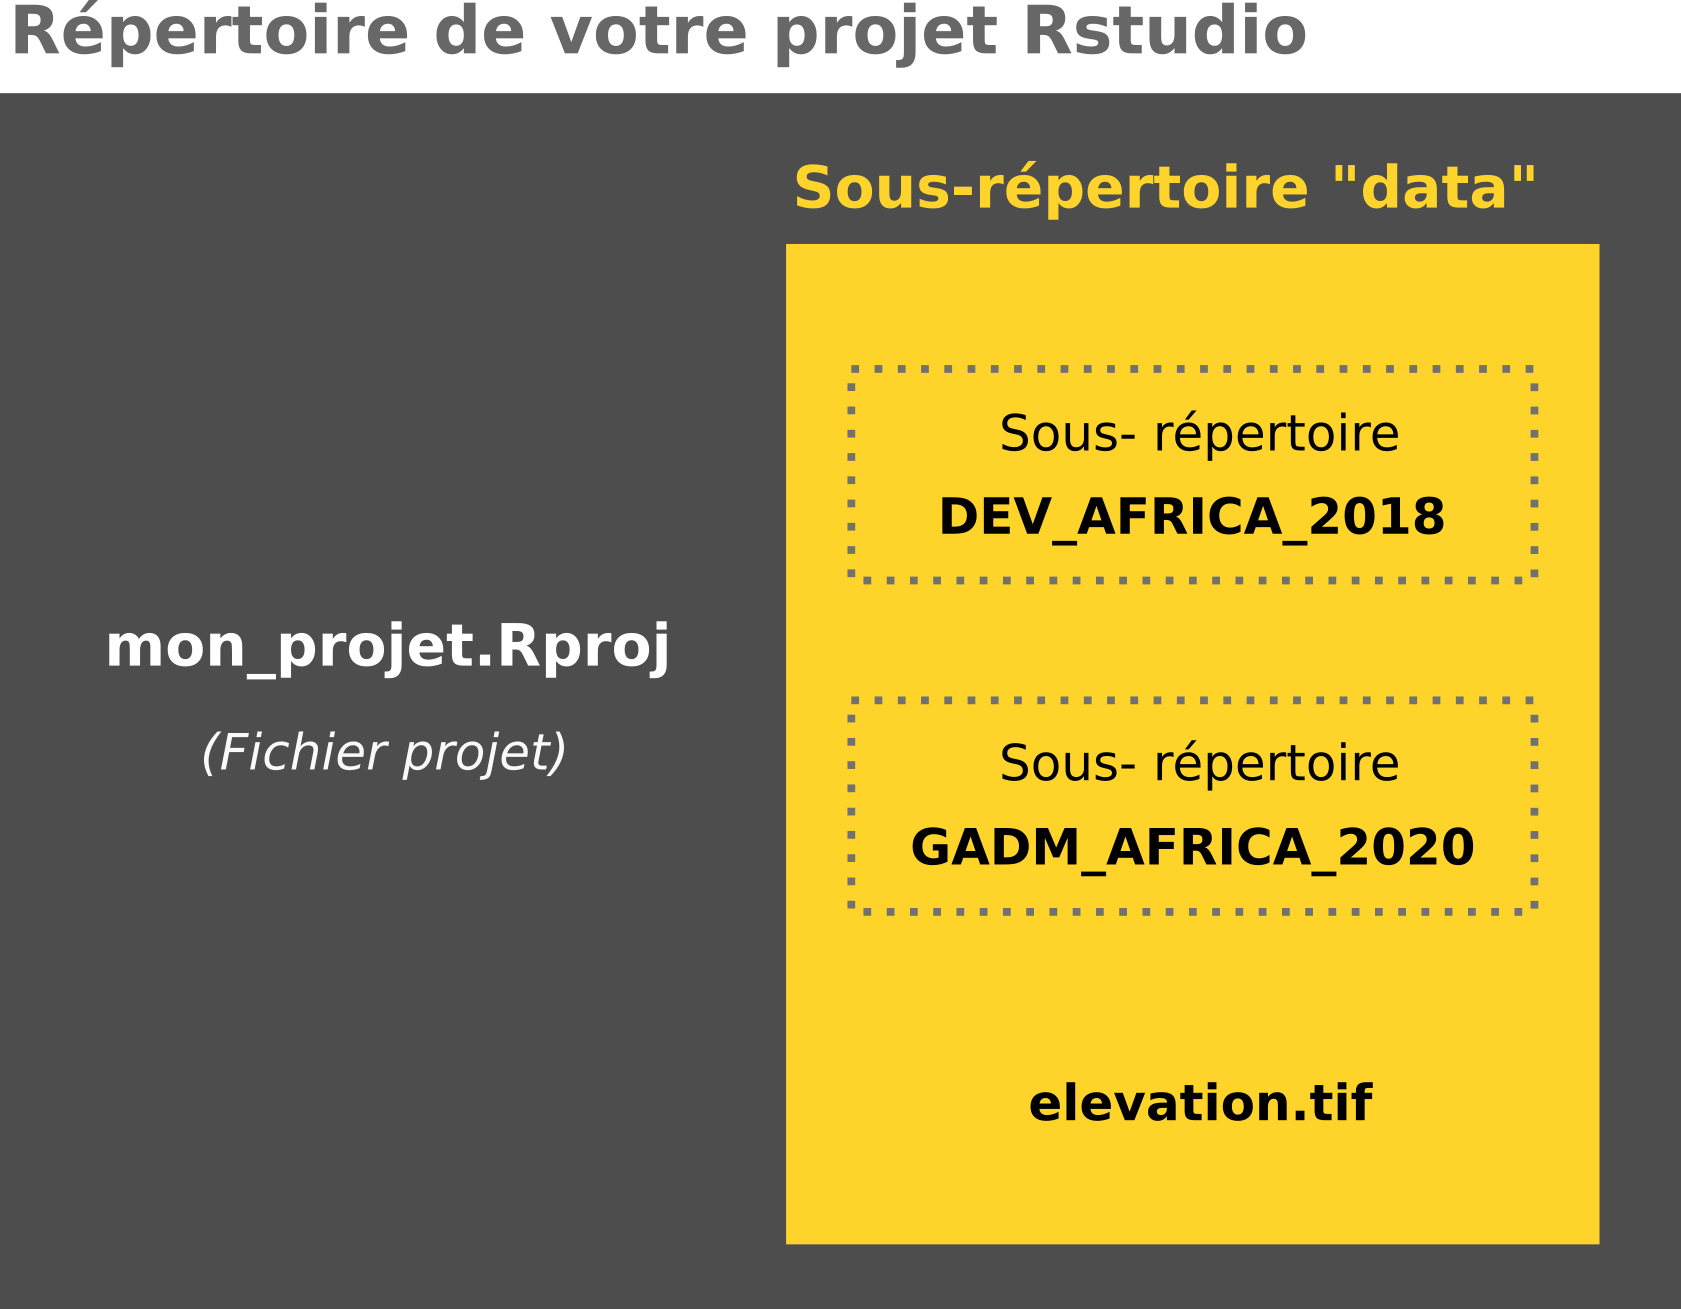
\includegraphics[width=0.7\textwidth,height=\textheight]{../img/folder.png}

}

\end{figure}

{4. Créez un script R à la racine de votre projet Rstudio}

\emph{File/New File/R script}

{5. Importer les fichiers suivants en utilisant les fonctions adéquates
:}

\begin{itemize}
\tightlist
\item
  data/DEV\_AFRIA\_2018/\textbf{afrika\_don.csv}\\
\item
  data/DEV\_AFRICA\_2018/\textbf{afrika\_don.xls} (1er onglet)\\
\item
  data/GADM\_AFRICA\_2020/\textbf{afrika\_map.shp}\\
\item
  data/\textbf{elevation.tif}
\end{itemize}

\begin{center}\rule{0.5\linewidth}{0.5pt}\end{center}

\begin{Shaded}
\begin{Highlighting}[]
\CommentTok{\# Pour importer un fichier csv (afrika\_don.csv)}
\FunctionTok{read.csv}\NormalTok{()}
\FunctionTok{read.csv2}\NormalTok{()}

\CommentTok{\# Pour importer un fichier Excel (afrika\_don.xls)}
\FunctionTok{library}\NormalTok{(readxl)}
\FunctionTok{read\_excel}\NormalTok{()}

\CommentTok{\# Pour importer un fichier ESRI Shapefile (afrika\_map.shp)}
\FunctionTok{library}\NormalTok{(sf)}
\FunctionTok{st\_read}\NormalTok{()}
\end{Highlighting}
\end{Shaded}

\begin{Shaded}
\begin{Highlighting}[]
\CommentTok{\# Import du fichier csv "afrika\_don.csv"}
\NormalTok{data\_from\_csv }\OtherTok{\textless{}{-}} \FunctionTok{read.csv2}\NormalTok{(}\AttributeTok{file =} \StringTok{"data/DEV\_AFRICA\_2018/afrika\_don.csv"}\NormalTok{)}

\CommentTok{\# Import du fichier xls "afrika\_don.xls"}
\FunctionTok{library}\NormalTok{(readxl)}
\NormalTok{data\_from\_xls }\OtherTok{\textless{}{-}} \FunctionTok{read\_excel}\NormalTok{(}\AttributeTok{path =} \StringTok{"data/DEV\_AFRICA\_2018/afrika\_don.xls"}\NormalTok{)}

\CommentTok{\# Importer du fichier shp "afrika\_map.shp"}
\FunctionTok{library}\NormalTok{(sf)}
\NormalTok{data\_from\_shp }\OtherTok{\textless{}{-}} \FunctionTok{st\_read}\NormalTok{(}\StringTok{"data/GADM\_AFRICA\_2020/afrika\_map.shp"}\NormalTok{,  }\AttributeTok{quiet =} \ConstantTok{TRUE}\NormalTok{)}
\end{Highlighting}
\end{Shaded}

\hfill\break
\hfill\break

Télécharger ce document format PDF



\end{document}
